% Trimmed decision tree (3 splits, 4 leaves).
% Layout: decision chain runs vertically; leaves branch to the right.
% Requires: \usetikzlibrary{shapes.geometric, arrows} (already in main.tex)
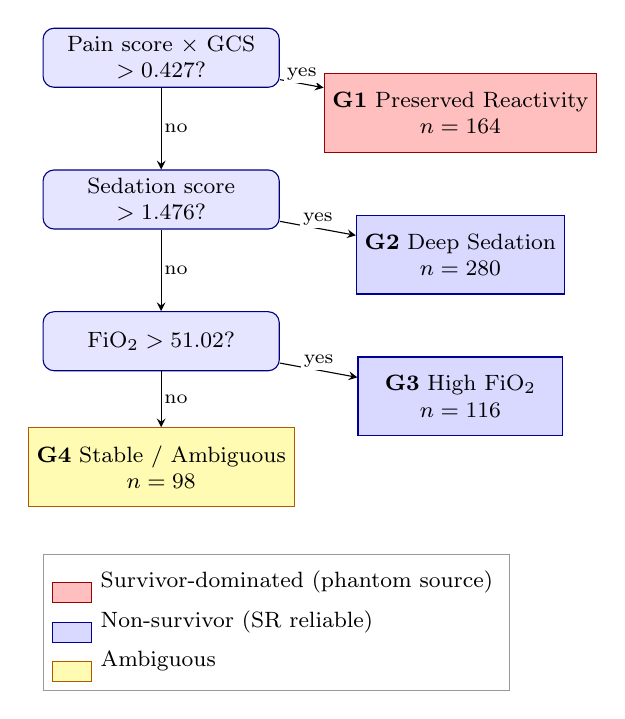
\begin{tikzpicture}[
    every node/.style={font=\footnotesize, align=center},
    decision/.style={rectangle, rounded corners, draw=blue!50!black,
                     fill=blue!10, minimum width=3.0cm, minimum height=0.75cm,
                     inner sep=2pt},
    leaf/.style={rectangle, draw=black!60, fill=gray!15,
                 minimum width=2.6cm, minimum height=1.0cm, inner sep=3pt},
    leaf phantom/.style={leaf, fill=red!25, draw=red!60!black},
    leaf reliable/.style={leaf, fill=blue!15, draw=blue!60!black},
    leaf ambiguous/.style={leaf, fill=yellow!30, draw=orange!70!black},
    edgelabel/.style={font=\scriptsize, fill=white, inner sep=1pt},
    >=stealth,
]

% ---------- Decision chain (vertical spine) ----------
\node[decision] (root) at (0, 0)
    {Pain score $\times$ GCS\\$> 0.427$?};

\node[decision] (n1) at (0, -1.8)
    {Sedation score\\$> 1.476$?};

\node[decision] (n2) at (0, -3.6)
    {FiO$_2 > 51.02$?};

% ---------- Leaves (right side) ----------
\node[leaf phantom] (g1) at (3.8, -0.7)
    {\textbf{G1} Preserved Reactivity\\$n=164$};

\node[leaf reliable] (g2) at (3.8, -2.5)
    {\textbf{G2} Deep Sedation\\$n=280$};

\node[leaf reliable] (g3) at (3.8, -4.3)
    {\textbf{G3} High FiO$_2$\\$n=116$};

% ---------- Final leaf (below spine) ----------
\node[leaf ambiguous] (g4) at (0, -5.2)
    {\textbf{G4} Stable / Ambiguous\\$n=98$};

% ---------- Edges ----------
\draw[->] (root) -- node[edgelabel, midway, above]{yes} (g1);
\draw[->] (root) -- node[edgelabel, right]{no}         (n1);

\draw[->] (n1)   -- node[edgelabel, midway, above]{yes} (g2);
\draw[->] (n1)   -- node[edgelabel, right]{no}          (n2);

\draw[->] (n2)   -- node[edgelabel, midway, above]{yes} (g3);
\draw[->] (n2)   -- node[edgelabel, right]{no}          (g4);

% ---------- Legend ----------
\matrix [draw=black!40, fill=white, inner sep=3pt,
         anchor=north west, font=\scriptsize] at (-1.5, -6.3) {
    \node[leaf phantom,   minimum width=0.5cm, minimum height=0.25cm] {}; &
        \node[anchor=west] {Survivor-dominated (phantom source)}; \\
    \node[leaf reliable,  minimum width=0.5cm, minimum height=0.25cm] {}; &
        \node[anchor=west] {Non-survivor (SR reliable)}; \\
    \node[leaf ambiguous, minimum width=0.5cm, minimum height=0.25cm] {}; &
        \node[anchor=west] {Ambiguous}; \\
};

\end{tikzpicture}
